\documentclass[10pt]{article}
\usepackage{comment}
\usepackage{listings}
\usepackage{graphicx}
\usepackage{psfrag}
\usepackage{amssymb}
\usepackage{amsmath}
\usepackage{algorithm2e}
\usepackage{caption}
\usepackage{epstopdf}
\usepackage{url}
\usepackage{fullpage}


%\usepackage{epsfig}
%\usepackage{subfigure}


\begin{comment}
\newtheorem{theorem}{Theorem}[section]
\newtheorem{proposition}[theorem]{Proposition}
\newtheorem{lemma}[theorem]{Lemma}
\newtheorem{corollary}[theorem]{Corollary}
\newtheorem{definition}[theorem]{Definition}
\end{comment}


\usepackage{enumerate}
\usepackage{float}
\usepackage{flafter}
\usepackage{psfrag}
\usepackage{overpic}
\usepackage{subfigure}
\usepackage{caption}
\usepackage{multirow}
\usepackage{array}

\usepackage{amsmath}

%\usepackage{graphicx}
%\usepackage{caption}
%\DeclareCaptionType{copyrightbox}
%\usepackage{subcaption}
%\usepackage[on]{auto-pst-pdf} % enable psfrag for pdflatex
%\usepackage{xcolor}


\usepackage{epsfig}



\usepackage{color}% Include colors for document elements (required for psfrag)

\newcommand{\psdir}{./sections}
\newcommand{\ldir}{./sections}
\newcommand{\fig}{./sections/fig}
\newcommand{\comm}[1]{}


\def\IL{{\it left}}
\def\IM{{\it middle}}
\def\IR{{\it right}}
\def\IB{{\it bottom}}
\def\IT{{\it top}}


\newcommand{\algref}[1]{Algorithm~\ref{#1}}
\newcommand{\defref}[1]{Definition~\ref{#1}}
\newcommand{\secref}[1]{Section~\ref{#1}}
\newcommand{\figref}[1]{Fig.~\ref{#1}}
\newcommand{\exref}[1]{Ex.~#1}
\newcommand{\tabref}[1]{Table~\ref{#1}}
\newcommand{\thmref}[1]{Theorem~\ref{#1}}
\newcommand{\propref}[1]{Proposition~\ref{#1}}
\newcommand{\efct}[1]{$\langle$ #1 $\rangle$}

\newcommand{\chapref}[1]{Chapter~\ref{#1}}

\newcolumntype{C}[1]{>{\centering\let\newline\\\arraybackslash\hspace{0pt}}m{#1}}


\newcommand{\atlasMgrid}{Atlas MultiGrid}
\newcommand{\cg}{$\cal{G}$}
\newcommand{\cgraph}{active constraint graph}
\newcommand{\sgraph}{stratification graph}
\newcommand{\cs}{$\cal{S}$}
\newcommand{\cd}{colldet}
\newcommand{\pconfig}{parametrized configuration}
\newcommand{\orient}{pose}
\newcommand{\point}{point}
\newcommand{\helix}{molecular composite}
\newcommand{\atom}{atom marker}
\newcommand{\dumbell}{dumbell}
\newcommand{\EASAL}{\texttt{EASAL}}
\newcommand{\Cr}{Cartesian realization}

\newcommand{\tns}{T} %total number of samples
\newcommand{\C}{C} %the collection of interesting atom pairs
\newcommand{\m}{m} %size of S
\newcommand{\stp}{s}


\newcommand{\tol}{$\tau$}
\newcommand{\AC}{A}
\newcommand{\mU}{M}
\newcommand{\aU}{atom marker}
\newcommand{\acg}{G}

\newcommand{\distall}{$C_1$}
\newcommand{\distexist}{$C_2$}

\newcommand{\acgW}{active constraint graph}
\newcommand{\acr}{active constraint region}
\newcommand{\distcons}{Distance Constraints}
%\def\acr{active constraint region}


\newcommand{\cover}{boundaries}


\newcommand{\aview}{atlas view}
\newcommand{\pview}{parametrized chart view}
\newcommand{\rview}{realization view} %configuration space view
\newcommand{\param}{parameter}
\newcommand{\idialog}{intervention dialog}
\newcommand{\ndialog}{node selection dialog}
\newcommand{\atlas}{\textit{atlas}}
\newcommand{\threeRealizable}{$3$-realizable}
\newcommand{\chart}{chart}
\newcommand{\toytwod}{Toy3}
%\newcommand{\toytwod}{Toy$\mathbb{R}^2$}
\newcommand{\toyCayley}{Toy2DCayleyExample}
\newcommand{\toyhelix}{6Atom}
\newcommand{\bighelix}{Toy20}
%\newcommand{\bighelix}{20Atom}
\newcommand{\ctwo}{\ref{eqn:preferredConstraints}}
\newcommand{\cone}{\ref{eqn:constraints}}
\newcommand{\MC}{MC~}
\newcommand{\MD}{MD~}
\newcommand{\custo}{region-specific}
% for lists
\renewcommand{\labelitemi}{$\bullet$}



\def\jorg#1{\textcolor{blue}{#1}}
\definecolor{brown}{RGB}{150,50,50}
\definecolor{pink}{RGB}{219, 48, 122}
\def\old#1{\textcolor{brown}{#1}}
% \def\aysegul#1{\textcolor{red}{#1}}
\def\mred#1{\textcolor{red}{#1}}


% for review
\definecolor{seagreen}{RGB}{48,178,139}
\definecolor{yelloworange}{RGB}{200,146,0}
\definecolor{purple}{RGB}{123,104,238}
%\definecolor{purple}{RGB}{147,112,219}
\definecolor{grayoned}{RGB}{0,0,255}
\definecolor{green2d}{RGB}{0,150,0}
\definecolor{plum}{RGB}{127,0,126}

\newcommand{\aysegul}[1]{{\color{blue}#1}}
\newcommand{\meera}[1]{{\color{magenta}#1}}
\newcommand{\troy}[1]{{\color{seagreen}#1}}
\newcommand{\rahul}[1]{{\color{cyan}#1}}
\newcommand{\joel}[1]{{\color{yelloworange}#1}}
\newcommand{\ruijin}[1]{{\color{plum}#1}}


%opening
\title{\EASAL~User Manual: \\User Interface and Functionalities}

\author{Aysegul Ozkan, Rahul Prabhu, Ruijin Wu, Troy Baker, \\James Pence, Jorg
Peters, Meera Sitharam \\ University of Florida}

 
\begin{document}

\maketitle
This user guide accompanies the \EASAL~software described in
\cite{Ozkan2014TOMS} which implements a suite of algorithms that elucidate the
structure and geometric properties of configuration spaces in molecular
assembly. The algorithms presented use new theoretical results by some
of the authors for: stratification of configuration
spaces, efficient sampling by convex
parametrization, and intuitive visualization. Technical concepts
and definitions required to use this software can be found in the main paper.


\section{Introduction}
 \EASAL\ elucidates the structure and geometric properties of configuration spaces in molecular assembly ~\cite{Sitharam:2012:EASAL, Ozkan2014MainEasal,
Wu2014Virus}. \EASAL\ implements algorithms that use new theoretical results, some of which are presented in ~\cite{Ozkan2014TOMS, Ozkan2014MainEasal, Gao, Sitharam:2012:EASAL}.
\EASAL~is open source and can be downloaded from \url{https://www.bitbucket.org/geoplexity/easal}.This user guide describes in
depth the features and options available in \EASAL.  The user can find a
detailed example of how to use the software in the README.md file which can be
found along with the source code. A video demonstrating \EASAL~in action is
available at \url{http://www.cise.ufl.edu/~sitharam/EASALvideo.mpg}.  Though
this version of the video is slightly dated in that it uses an older version of
the software (only the GUI in the Atlas View has changed since), it should
serve as a good resource to gain familiarity with \EASAL. A newer version of
the video is being created and will be uploaded soon to
\url{http://cise.ufl.edu/~rprabhu/EASALvideo}.


\section{Software Functionalities}
This section introduces the main functionalities of EASAL and gives details of how it has been implemented in the software.
\subsection{Input}
The input to EASAL consists of the following:
\begin{itemize}
\item Two rigid molecular units.
\item The pairwise component of the potential energy or enthalpy function.
\item The global, non-pairwise component of the potential energy is modeled as the angle
constraint between the principal axes of the two rigid molecular units.
\end{itemize}

These can be specified in the input window which the user is presented with when EASAL is first run (see Fig. ~\ref{Input}).

\begin{figure}[h]
\centering
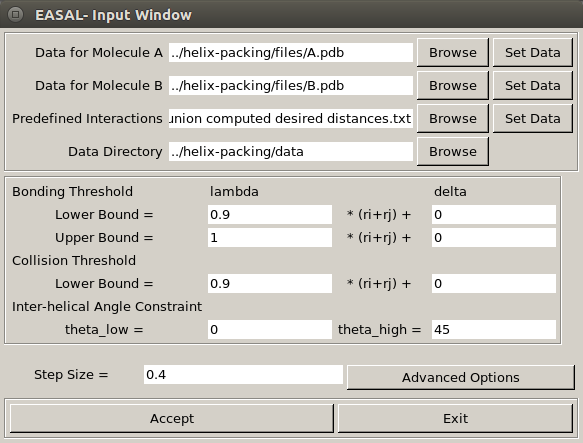
\includegraphics[scale=0.5] {fig/Input.png}
\caption{Input Window}
\label{Input}
\end{figure}

\begin{itemize}
\item \textbf{Data for Molecule (A/B)} This accepts the molecular data
		describing the molecular composites and their 3D structure pdb format.
		The user can either type in the location of the input molecular files
		or select it using the browse option. Once a file has been selected,
		the `set data' option allows the user to edit the input molecular data
		before starting sampling.
\item \textbf{Predefined Interactions:} Predefined Interactions is information
		about the minimum and maximum distances between atom pairs
		participating in the bonding. The input file for this can either
		specify pair-wise distance for each atom pair participating in the
		reaction from either molecules or only specify distances of atoms the
		user is interested in.
\item \textbf{Inter-helical Angle Constraint:} This specifies the upper and
		lower bound for angle constraints between the two atoms. This forms
		the global component of the energy function.

\end{itemize}

\subsection{Geomtrization}
The Lennard-Jones potential function is typically discretized to
take constant values on three intervals where the repulsive forces dominate, the at-
tractive forces dominate and neither dominates. All these bounds are specified as part
of the input to the assembly model for each pair of atoms. Using the Input window, the user can specify these distances. 

\begin{itemize}

\item \textbf{Bonding Threshold:} This is the range of distances between atoms
		where bond formation is feasible (i.e., the attractive forces dominate). 
		This is given as $\lambda*(r_i+r_j)
		\pm \delta$. Where $\lambda$ is specified by the lambda text field in
		the input window and $\delta$ is specified by the delta text box in the
		input window. $r_i$ and $r_j$ are the radii of the atoms participating
		in the reaction. 

\item \textbf{Collision Threshold:} This is the minimum distance between atoms
		below which atoms will collide. This too is given as $\lambda*(r_i+r_j)
		\pm \delta$.

\end{itemize}

\subsection{Stratification}

The Atlas View visualizes the stratification of an assembly configuration
space. Strata of each dimension for the assembly constraint system are visually
represented as nodes of one color (see Fig. ~\ref{AtlasView}). The
stratification is a directed acyclic graph where each node represents an active
constraint region represented by an active constraint graph. Edges indicate
containment in a parent region one dimension higher.

The Atlas View shows the atlas as it is being built, as a dynamic forest of
trees.  It provides controls that allow the user to do real-time intervention
at any stage of the sampling process; to halt, redirect, and resume the
sampling process and to access the atlas for different queries or views.


\begin{figure}[hp]
\centering
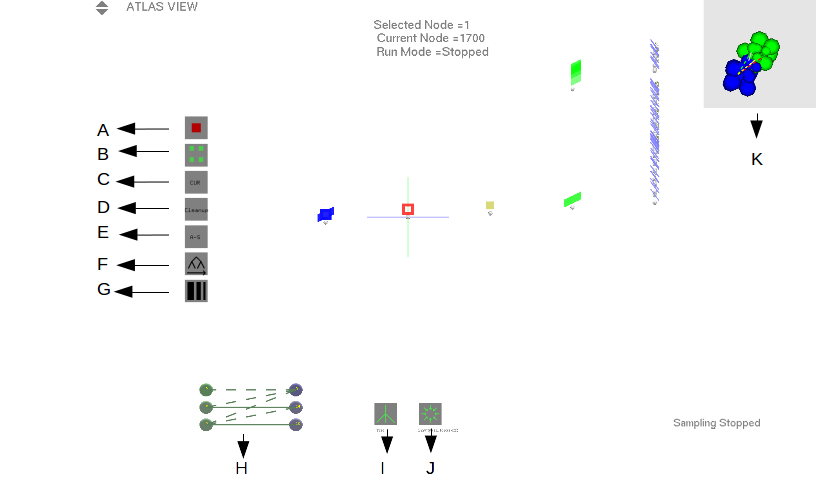
\includegraphics[width=1.\textwidth] {fig/AtlasView.png}
\caption{The Atlas View in \EASAL~. (A) Button to stop the sampling. (B) Button
to start the constraint selection dialogue box. (C) Button to continue sampling
the current tree. (D) Button to Clean Up Sampling. (E) Button to run EASAL in
the Auto-Solve mode. (F) Button to start exploring the Atlas in a breadth first
fashion. (G) Button to refine the sampling using a smaller step size. (H)
Active Constraint graph of the node selected. The spheres with the indices
denote the atoms. A thick line between the atoms indicates a bond and a dotted
line indicates a parameter. (I) Button to toggle Tree View. (J) Button to
toggle Gravity. (K) Cartesian realization of the current node.}
\label{AtlasView} \end{figure}

\subsubsection{Sampling}
\EASAL~generates an \emph{atlas}~\cite{Sitharam:2012:EASAL} of the configuration
space. This atlas is a forest of trees where each $d$-dimensional node represents
an active constraint region of dimension $d$. Each tree in the atlas has has either
a four or five dimensional root node and each successive level of the tree has nodes of
one dimension lesser than the previous level. The atlas is
generated by sampling the configuration space in any of the following sampling modes.

\begin{itemize}
\item \textbf{Auto-Solve:} This is the default sampling mode. When starting
		afresh in this mode, \EASAL~generates all possible root nodes of
		either four or five dimensions depending on the user input. Then it
		proceeds to recursively sample all these nodes till the atlas generation
		is complete. If there is a partially generated atlas, this mode of
		sampling completes	 the unfinished trees and then proceeds to sample
		all the other root nodes.
\item \textbf{Current Tree:} In this mode of sampling, \EASAL~starts from the
		node currently selected and samples its tree to completion.
\item \textbf{Clean Up:} In this mode, \EASAL~samples all incomplete trees to
		completion.
\item \textbf{Ad-hoc:} In this mode, the user can select any node of any
		dimension using the ``constraint selection dialogue box'' and sample
		the sub-tree rooted at that node.
\item \textbf{Breadth First:} While all other sampling modes sample the tree
		depth first, this mode samples the tree breadth first. Starting from a
		selected node, this mode samples the sub-tree rooted at that node in a
		breadth first fashion.
\item \textbf{Refine Sampling:} The user can use this mode for a more refined
		level of sampling. In this mode, we re-sample all the completed nodes
		with a step size equal to half the original step size.
\end{itemize}



\subsection{Convex Cayley Parametrization}

The space view shows the active constraint region in the Cayley parametrized
chart representation for a particular node.  Clicking a node loads its active
constraint region to RAM and the space view is brought when user press enter
key. The parametrized chart view (Fig. ~\ref{SpaceView}) shows green cubes (such
that the cube size is proportional to the step size chosen) where parameters do
not result in collision. Clicking a cube displays, in the upper right corner, a
Cartesian realization associated with the parameter values (respec- tive Cayley
point). (EASAL can also display parameters resulting in irreconcilable inter-
molecular collisions or ones that are not realizable.) For more than three
dimensions, arrow-controlled sliders select and display 3D slices. Since
interior points are easily occluded, the third dimension can also be switched
to a slider. The left side of the view enumerates newly formed lower
dimensional boundaries of the active constraint region and enumerates
color-coded boundaries.

\begin{figure}[h]
\centering
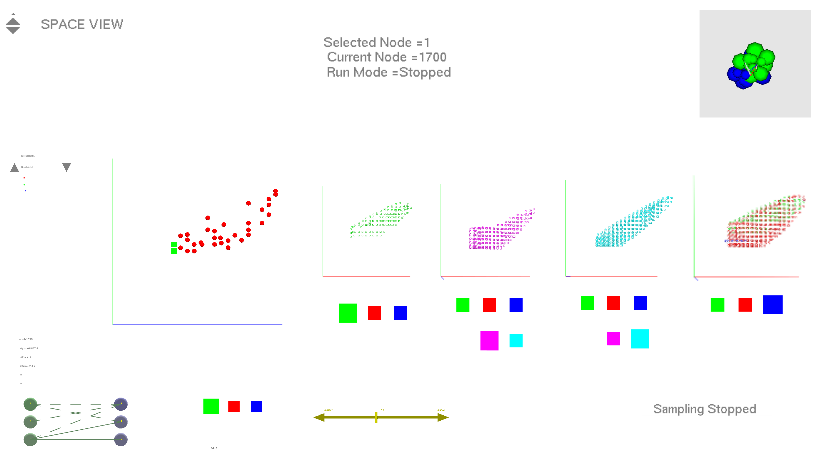
\includegraphics[width=\textwidth] {fig/CayleySpaceView.png}
\caption{Cayley Space View. The points outside the box show the boundary
points. The points in the box show the various cayley points. From left to
right Good points, Collision points, points which violate the steric
constraints and all the points sampled.}
\label{SpaceView}
\end{figure}


\subsection{Cartesian Realization}
The realization view shows the active constraint region in the Cartesian
realizations representation for a particular node. The realization view 
(Fig. ~\ref{RealizationView}) shows realizations with
constraints and parameters displayed as lines. Valid realization flips are
shown on the lower right side of the view.  One option to view the valid
parameters in the order of detection is via ‘video controls’ (bottom right)
with reverse, pause, play and stop options.


\begin{figure}[h]
		\centering
		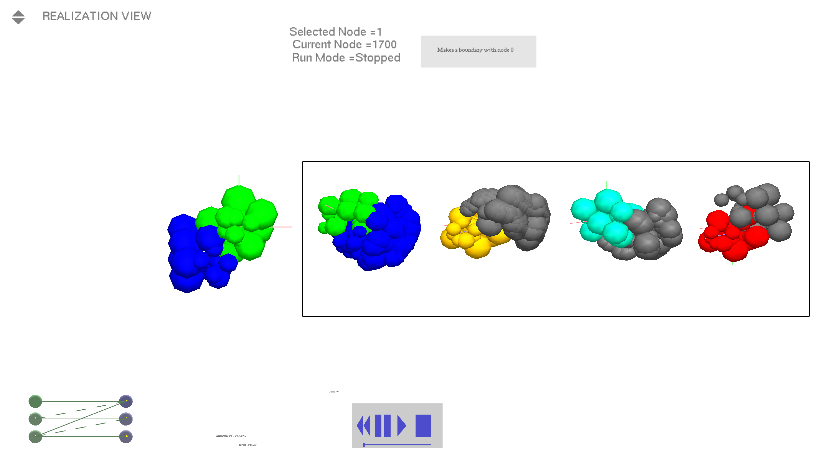
\includegraphics[width=\textwidth] {fig/RealizationView.png}
		\caption{Realization View. The images in the box show the different
		realizations along different boundaries.}
		\label{RealizationView}
\end{figure}



\section{User Interface}
\subsection{Input Window}
This section describes all the input options not previously described.

\begin{itemize}

\item \textbf{Data directory:} This is the directory where the atlas is stored.
		If \EASAL~finds a partially generated atlas at this location, it
		presents the user with 3 options. The user can choose to (i) Continue
		sampling the old atlas, in which case the old atlas is loaded. (ii)
		Overwrite the existing data and start fresh sampling. (iii) Go back and
		choose a different location for the atlas.

\item \textbf{Step size:} This is the step size used for sampling the Cayley
		Space.

\item \textbf{Advanced Options:} This gives a set of advanced options to the
		user.

\begin{figure}[h]
\centering
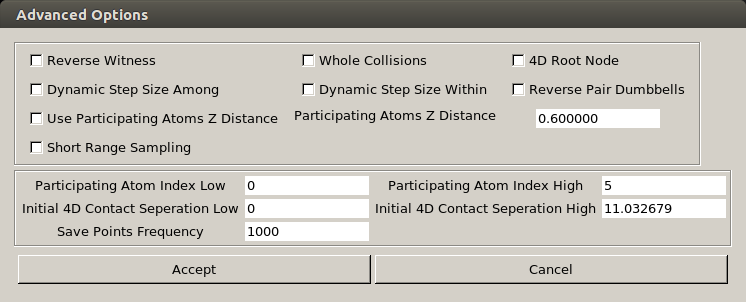
\includegraphics[scale=0.5] {fig/AdvancedOptions.png}
\caption{Advanced Options Window}
\label{Input}
\end{figure}

\begin{itemize}
\item \textbf{Reverse Witness:} Some nodes in the atlas do not have convex
		parameterizations and hence cannot be  directly populated. However
		these can be populated indirectly from a child node encountered through
		another path. When this option is enabled, \EASAL~adds a witness point
		to all parent nodes found this way.  
\item \textbf{Whole Collisions:} By default, \EASAL~checks for collisions
		between every pair of atoms. When the input atoms are large, this may
		not be feasible. Whole Collisions provides a way of checking for
		collisions between a group of atoms.
\item \textbf{4D Root Node:} Choosing this option makes the root nodes in the
		atlas correspond to  4 dimensional active constraint regions instead of
		the default 5 dimensional regions.
\item \textbf{Dynamic Step Size Among/Within:} When chosen, uses a step size
		dynamically determined based on the volume of the region to be sampled
		instead of the user supplied step size. Among chooses dynamic step size
		for every parameter. Within choose a dynamic step size just for one
		parameter.
\item \textbf{Reverse Pair Dumbbells:} For the $4D$ case, by default we choose
		the initial contacts so that the atom with the lower number on one
		molecule pairs up with the atom with the lower number on the other
		molecule. Using Reverse pair dumbbells removes this restriction.
\item \textbf{Use Participating Atom Z Distance:} This option limits the z-axis
		distance between atoms participating in the bonding.
\item \textbf{Participating Atom Z Distance:} This option specifies the
		threshold for participating atom z-distance.
\item \textbf{Short Range Sampling:} This allows for flexible sampling.
\item \textbf{Participating Atom Index Low/High:} These force the constraints
		to be picked from the middle of the molecules. Low and High are the
		atom numbers between which the user wants the constraints to be picked.
\item \textbf{Initial 4D Contact Separation Low/High:} In the $4D$ case, this
		is the maximum separation between atoms in the same molecule that form
		a dumbbell.
\item \textbf{Save Points Frequency:} The frequency with which sampled points
		are saved to a file in the data directory.

\end{itemize}
\end{itemize}

Clicking Accept on the Input Window takes the user to the Atlas View of the
software where sampling starts in the default Auto-Solve mode.

\subsection{Atlas View}

\begin{itemize}
\item \textbf{Stop Sampling:} Clicking this button stops the sampling of the
		Atlas and presents options to redirect the sampling.
\item \textbf{The Constraint Selection Dialogue box }(see figure~\ref{DSD})
		allows the user to select a particular node from the atlas and start
		sampling from that node. This feature gives users the flexibility to
		explore regions of the graph that is more relevant to them. The user
		can select a node by either specifying a node number or by specifying
		active constraints between the molecules. The spheres with the indices
		denote the atoms. A thick line between the atoms indicates a bond
		participating in the reaction. Here, the first constraint is mandatory
		and hence does not have a `connect' check box next to it. The rest of
		the Active constraints are optional and the user may choose up to six.
		\begin{figure}[h]
				\centering
				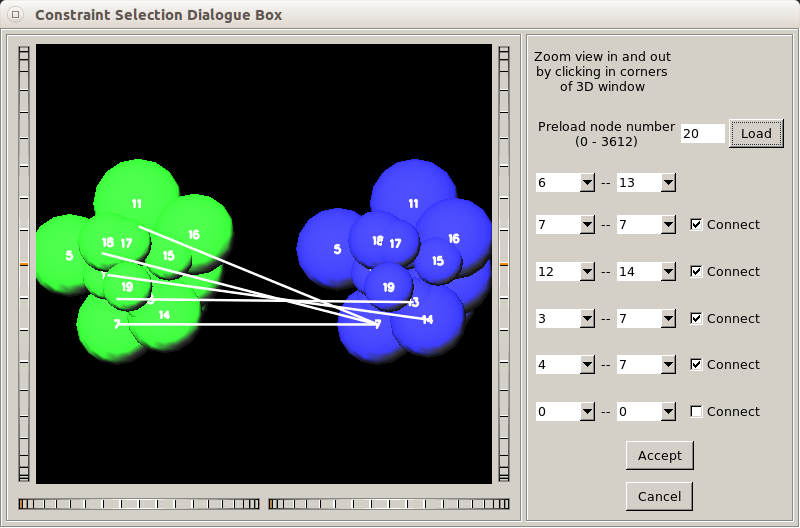
\includegraphics[scale=0.5] {fig/DumbbellSelection.png}
				\caption{Constraint Selection Dialogue}
				\label{DSD}
		\end{figure}

\item \textbf{CUR:} On clicking this, the sampling starts from the node that is
		currently selected and ends when the tree in which the node is present
		is fully sampled.
\item \textbf{Cleanup:} Clicking this completes sampling on all the partially
		sampled trees.
\item \textbf{A-S:} A-S stands for Auto-Solve. This button starts sampling in
		the Auto-Solve mode.
\item \textbf{BFS:} Clicking this button forces \EASAL~to explore the atlas in
		a breadth first fashion which it otherwise does in a depth first
		fashion.
\item \textbf{Refine Sampling:} On clicking this button \EASAL~starts sampling
		with half the current step size.
\item \textbf{Tree:} Clicking `Tree' after selecting a particular node from the
		atlas shows us only those nodes that are either the ancestors or the
		descendants of the node selected.
\item \textbf{Gravity:} \EASAL~implements a spring-repulsion algorithm that
		yields a spacious layout of the nodes in  atlas. This button
		enables/disables the spring-repulsion algorithm.
\item \textbf{Keyboard Shortcuts:}
		\begin{itemize}
				\item \textbf{`+'} - Zoom into the atlas.
				\item \textbf{`-'} - Zoom out of the atlas.
				\item \textbf{`f'} - Toggle forces. \EASAL~implements a spring
						repulsion algorithm to display the atlas. This toggles
						the spring repulsion on and off.
				\item \textbf{`l'} - Enables level alignment. Enabling this
						arranges the nodes of the atlas according to their
						dimensions.
				\item \textbf{`i'} - Align view to x axis.
				\item \textbf{`j'} - Align view to y axis.
				\item \textbf{`k'} - Align view to z axis.
				\item \textbf{`t'} - Toggles the tree view. When the tree view
						is on, it shows only the tree the the currently
						selected node is part of. When it is off, it shows the
						entire atlas. This can also be achieved by clicking the
						Tree control at the bottom.
				\item \textbf{`1'} - Toggles the display of node numbers.
				\item \textbf{`w'} - Toggle hide/show atlas edges.
				\item \textbf{`a'} - Toggles between showing and not showing
						nodes with no realizations. By default, nodes which do
						not have any realizations are not shown in the atlas.
				\item \textbf{`s'} - \EASAL~saves the atlas periodically
						depending on the `save points frequency' set by the
						user. Pressing `s' forces it to save the atlas to the
						disk even if it is in between two save cycles.
		\end{itemize}
\end{itemize}



\subsection{Space View}
This section discusses all the user options available to explore the Cayley Space.
\begin{itemize}
		\item \textbf{View dim:} Clicking on this allows the user to step
				through points in the Cayley space in each dimension. A slider
				is provided to visualize points in higher dimensions.  \item
				\textbf{Boundaries:} allows the user to inspect the boundaries
				of the Cayley space.  Different colors are used to represent
				different boundaries in the Cayley Space. The user can step
				through each of the boundaries using arrows provided.
		\item \textbf{Categorization of Cayley points:} In the Calyey Space
				View, initially green points are shown which correspond to all
				the realizable points in the cayley space. Clicking on the Red
				square at the bottom, shows the the points that have collision.
				Clicking the red also shows two more options viz., cyan and
				pink. The Cyan points represent the points which have angle
				collision and the pink points represent points which have
				distance collision.
		\item \textbf{Keyboard Shortcuts:}
				\begin{itemize}
						\item \textbf{`6'} - Switches the sliders to 6-d view.
						\item \textbf{`3'} - Switches the sliders to 3-d view.
						\item \textbf{`2'} - Switches the sliders to 2-d view.
						\item \textbf{`b'} - Toggles showing the boundary points.
						\item \textbf{`,'/`$<$'} - Cycles through the different
								boundary points downwards.
						\item \textbf{`.'/`$>$'} - Cycles through the different
								boundary points upwards.
				\end{itemize}
\end{itemize}

\subsection{Realization View}
This section discusses all the user options available to explore the realization.
\begin{itemize}
		\item Pressing `v' generates a sweep of all possible realizations for
				the node selected.  Pressing `v' again generates an instance of
				realization for the Cayley Point selected in Space View.  The
				user can step through all possible flips by pressing the up and
				down arrow keys.
		\item Clicking on boundaries generates the sweep of all realizations
				along different boundaries of the Cayley space.
		\item Video controls at the bottom allow for animation of all the
				realizations and their flips.
		\item Keyboard Shortcuts
				\begin{itemize}
						\item \textbf{`v'} - Generates a sweep of all possible
								realizations. 
						\item \textbf{numbers 0-7} - Jump to flip number
								pressed. 
						\item \textbf{`s'} - Toggle show and hide the whole
								s-tree.
						\item \textbf{`l'} - Show the bonds between the atoms.
				\end{itemize}
\end{itemize}


\begin{figure}[hp]
\centering
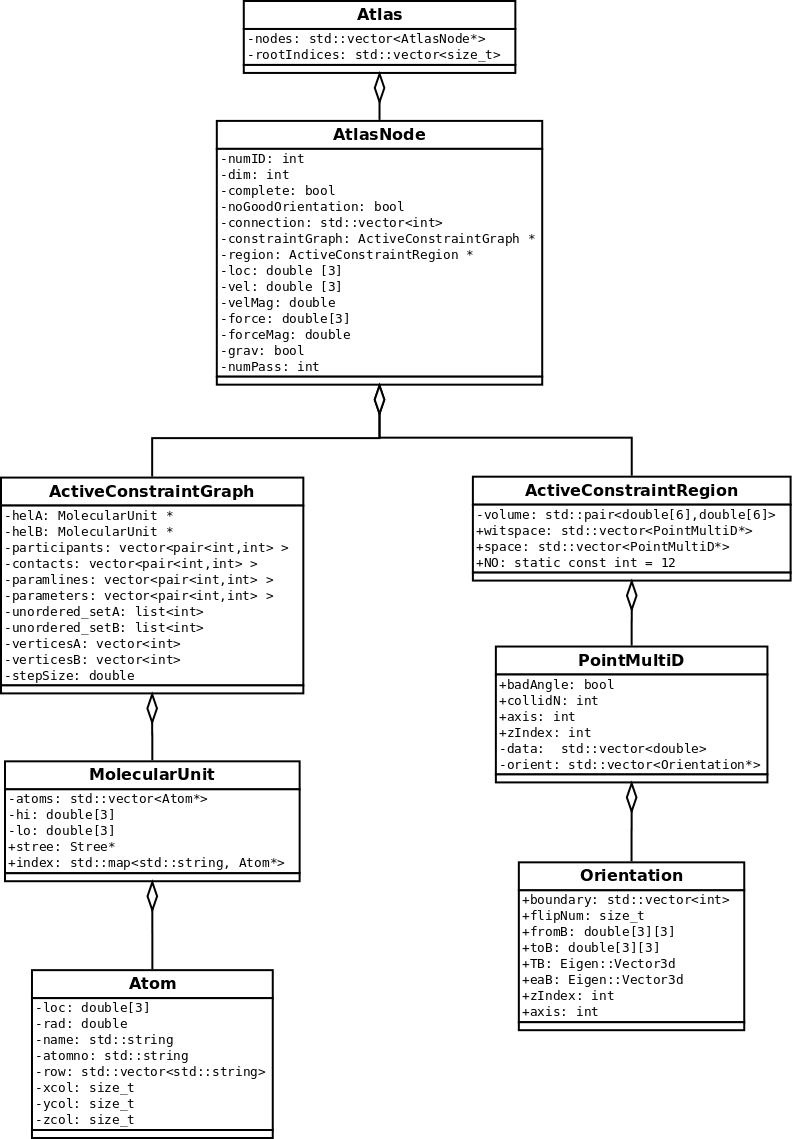
\includegraphics[scale=0.3] {fig/EASAL_UML.png}
\caption{\EASAL~UML Diagram}
\label{UML}
\end{figure}



\section{\EASAL~Software Architecture and Pseudocode}
\label{sec:architecture}
\section{Major Classes of \texttt{EASAL}}
\label{sec:classes}
\begin{figure}[h]
\centering
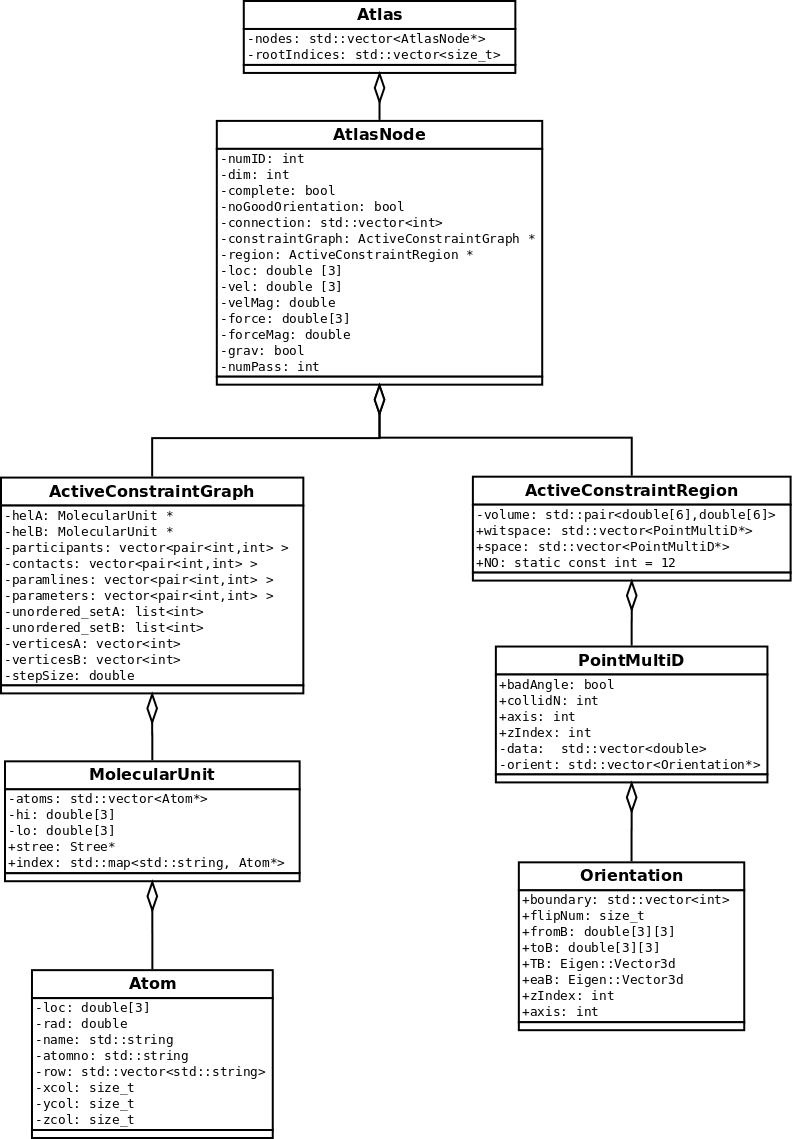
\includegraphics[scale=0.3] {fig/EASAL_UML.png}
\caption{EASAL UML Diagram}
\label{UML}
\end{figure}


\figref{UML} gives an overview of the structure of the major classes of EASAL.
Each of these classes are explained in the subsections below.

\subsection{AtlasBuilder} 

The AtlasBuilder class populates the ActiveConstraintRegion for each
activeConstraintGraph by sampling inside the boundaries of its ConvexChart. 
It creates and explores only regions that contain at least one Cartesian
realization. 

\begin{algorithm} [htbp]
 \SetKwInOut{Input}{input}\SetKwInOut{Output}{output}

 {\bf sampleAtlasNode}\\
 \Input{atlasNode: node}
 \Output{Complete sampling of the atlasNode and all its children}
 \BlankLine
 \LinesNumbered
	$H$ = node.activeConstraints\\
	$G_H$ = node.activeConstraintGraph\\
	\If{ $G_H$ is minimally rigid}
		{stop;	}
	$F$ = complete3Tree($G_H$)\\
	
	$C$ = computeConvexChart($G_H$, $F$)\\

	\For{ each cayleyPoint $p$ within convexChart $C$ }
	{
		$R$ = computeRealizations($p$)\\

		\For{ each realization $r$ in $R$}
		{
			\If{!aPosterioriConstraintViolated($r$)}
			{
				\If{ isBoundaryPoint($r$) \&\& hasNewActiveConstraint($r$, $G_H$) }
				{
					$e$ = newActiveConstraint($r$, $G_H$);\\
					$G'$ := $G_H \cup \{e\}$ ;\\
					\If{ $G'$ is not already present in the current atlas}
					{
						childNode = new atlasNode($G'$)\\
						sampleAtlasNode(childNode);\\
					} \Else{
						childNode = findNode($G'$);
					}
					node.setChildNode(childNode);
				} 
			}
		}
	}

	\caption{High level EASAL pseudocode}
\label{alg:sampleAtlasNode}
\end{algorithm}


\noindent \textbf{Major Attributes:} 
\begin{itemize}
		\item  \textbf{rootGraphs}: The set of all possible 4D or 5D
				ActiveConstraintGraphs of the root nodes
				generated before sampling.
		\item  \textbf{atlas}: An atlas object that is populated by the
				AtlasBuilder by sampling. This object is shared between front-end and
				back-end of the algorithm.
\end{itemize}

\noindent \textbf{Major Methods:}
\begin{itemize}
		\item  \textbf{startAtlasBuilding()}: For each of the generated root graph, 
				creates an atlasNode labeled with a contact graph $G_F$ where $F$ is the
				set of contacts. Then calls the recursive sampleTheNode method 
				for each of the root atlas nodes.
		\item  \textbf{sampleTheNode(atlasNode)}: The exploration of the atlas
				is done by the recursive \textbf{sampleAtlasNode} algorithm (see Algorithm 
				\ref{alg:sampleAtlasNode})
				using one of the generated atlas root nodes as input. This
				algorithm is implemented by the sampleTheNode method. Using
				depth first search this algorithm samples the atlas node and
				all its descendants. 
				
				\textbf{Base case of recursion:} If active constraint graph $G_H$ of the 
				node is minimally rigid i.e., the active constraint region is 
				0-dimensional, we have no more sampling to do, return.
				
				\textbf{The recursion step:} If $G_H$ is not minimally rigid, we use the
				\textbf{complete3Tree} algorithm to find find a set of parameters $F$ so 
				as to form a maximal 3-tree to leverage the convex parametrization theory~
				\cite{SiGa:2010}. This also ensures that $H \cup F$ is minimally rigid and 
				easily realizable. 
				
				The method computeConvexChart shown in the pseudocode finds the convex 
				chart for the parameters $F$ is done by the ConvexChart class explained 
				later. Method ComputeRealizations computes the realization for a 
				Cayley point and is done by the findRealizations method in the software. 
				The aPosterioriConstraintViolated method which checks for angle and steric 
				violations is implemented in the ConstraintCheck class explained later.
				Next we make a call to the findBoundary to detect boundaries and
				newly active constraints.
				

		\item  \textbf{determineStepSizeDynamically()}: Finds out the step size $s$
				given $T$, the total number of samples. Each 5D atlas node has its
				own $s$ computed by using the volume of the Cayley parameter space of the
				node over total number of samples per node. The volume of the
				Cayley parameter space of the node is approximately computed by
				exhaustive sampling within the exact chart without considering
				any constraints. The number of samples per node roughly can be
				computed by $T$ over total number of root(starter) atlas
				nodes, $m$. The number of samples in child nodes are negligible
				since the volume of regions in low dimensional nodes are
				negligible compared to the regions of high dimensional nodes.
		
		\item  \textbf{findBoundary()}: Boundary detection ensures that sampling 
				stays in the feasible region and minimizes discarded samples. 
				The findBoundary method which detects boundary points, checks 
				for newly formed active constraints and makes function calls
				which in turn call sampleTheNode for a child region.
		
\end{itemize}

\subsection{Atlas} 
The `Atlas' class stores the directed acyclic graph that represents the relationship between active constraint regions.

\noindent \textbf{Major Attributes:}
\begin{itemize}
		\item \textbf{nodes}: A vector of all AtlasNodes. 
		\item \textbf{rootIndices}: The indices of all the root nodes in the atlas.
\end{itemize}

\noindent \textbf{Major Methods:}
\begin{itemize}
		\item \textbf{search(node)}: Uses depth first search on the atlas to check
				whether the node exists in the atlas or not. It is used to avoid
				repeated sampling of the same region. The time complexity of
				the search is $O((\text{depth of the tree})) = O(6(k-1)) $ which in our 
				case is $O(1)$ since we fix $k$ to be 2.
\end{itemize}


\subsection{AtlasNode} 
AtlasNodes make up the Atlas. Each AtlasNode represents an active constraint region
reperesented by an ActiveConstraintGraph.

\noindent \textbf{Major Attributes:}
\begin{itemize}
		\item \textbf{acg}: The active constraint graph corresponding to the node.
		\item \textbf{region}: The set of Cayley points in the active region.
		\item \textbf{connection}: The id of the nodes in the atlas that
				represent the boundary of this node's region.
\end{itemize}

\subsection{ActiveConstraintGraph} 
The ActiveConstraintGraph class is used to store the set of active constraints.

\noindent \textbf{Major Attributes:} 
\begin{itemize}
		\item  \textbf{activeConstraints}: The set of point index pairs that represent 
				contacts.
		\item  \textbf{verticesA}: Participating points from first point set.
		\item  \textbf{verticesB}: Participating points from second point set.
		\item  \textbf{parameters}: A vector of point index pairs that represent parameters.
\end{itemize}

\noindent \textbf{Major Methods:}
\begin{itemize}
		\item  \textbf{completeTo3by3Graph()}: Adds points to make sure there
				are at least 3 points from each point set so that the graph is
				realizable. While choosing additional points, it has 2 options,
				choosing the points closest to each other or the points that lead
				to a user specified angle.
\end{itemize}


\subsection{ActiveConstraintRegion} 
The ActiveConstraintRegion class contains the set of feasible Cayley points generated
by sampling.

\noindent \textbf{Major Attributes:} 
\begin{itemize}
		\item  \textbf{space}: The set of feasible Cayley points.
		\item  \textbf{witspace}: The set of feasible witness Cayley points
				obtained from an ancestor node.
\end{itemize}

\noindent \textbf{Major Methods:}
\begin{itemize}
		\item  \textbf{convertSpace(activeConstraintRegion)}: Re-parametrizes
				a region using an input region’s parameters. This method
				converts each Cayley point in the input activeConstraintRegion
				to the Cayley point parametrized by the input region's
				parametrization.
\end{itemize}


\subsection{CayleyPoint} 
The CayleyPoint class represents a multi-dimensional point in the Cayley parameter space
and stores the corresponding Cartesian space orientations of the point set.

\noindent \textbf{Major Attributes:}
\begin{itemize}
		\item  \textbf{data}: Values of the Cayley parameters (non-edge
				lengths). \item  \textbf{orients}: The set of Cartesian space
				Orientations of the point set that were computed by
				realizing the active constraint graph with the given length of
				the edges and non-edges.
\end{itemize}

\subsection{Orientation} 
The Orientation class is the Euclidean transformation of point set. The
Orientation class stores only the information necessary to compute the
transformation matrix that will yield a Cartesian realization for the entire
point set.

\noindent \textbf{Major Attributes:} 
\begin{itemize}
		\item  \textbf{FromB}: Cartesian coordinates of three points from the
				first point set before the transformation.
		\item  \textbf{ToB}: Cartesian coordinates of three points from the
				second point set after the transformation.
		\item  \textbf{connections}: The set of node indices that this
				orientation belongs to. An orientation be on the
				boundary of multiple regions.
\end{itemize}


\subsection{CayleyParameterization} 
The CayleyParameterization class chooses non-edges in an ActiveConstraintGraph
that convert the graph into complete 3-tree. Those non-edges are called the
parameters. The complexity of the sampling algorithm varies based on the
choice of non-edges and the order in which they are fixed.

\noindent \textbf{Major Attributes:} 
\begin{itemize}
		\item  \textbf{partial3tree}: A boolean variable indicating whether
				an ActiveConstraintGraph is partial 3-tree or not.
		\item  \textbf{parameters}: The set of points pairs that represent
				non-edges. 
		\item  \textbf{tetrahedra}: The ordered tetrahedron set that helps in 
				defining the order of parameters that is required
				during the sampling procedure. This data is later passed to
				ConvexChart and CartesianRealizer to help in their computations. 
		\item  \textbf{updateList}: Adjacency map containing the dependency of
				parameters. It provides the set of parameters whose range will
				be updated when one of the parameters is fixed.
		\item  \textbf{boundaryComputationWay}: Inequalities that express the
				range of a parameter can be classified into either a linear or
				non-linear class. This variable is the characterization of the
				parameter that tells what inequality is needed to compute
				the parameter range i.e., triangular or tetrahedral inequality. 
		\item  \textbf{complete3trees}: The set of complete 3 trees.
\end{itemize}

\noindent \textbf{Major Methods:}
\begin{itemize}
		\item  \textbf{defineParameters()}: The parameters of an active
				constraint graph are selected as maximal 3-realizable (3-tree)
				extensions by leveraging the convex parametrization theory.
				\cite{SiGa:2010}. It creates a look-up table containing all possible 
				complete 3-trees. We find a graph in the look-up
				table so that active constraint graph is a proper subset of either the 
				graph or one of its isomorphisms.
		\item  \textbf{parameterMinDeviation()}: An alternate way to pick
				the parameters for 5D regions is by ensuring that the range
				of each parameter is similar. The aim here is to sample more
				uniformly in the Cartesian space. 
		\item  \textbf{built3tree()}: The 3-tree formed by starting with a
				4-vertex complete graph and repeatedly adding vertices in
				such a way that each added vertex is edge-connected to the face
				of a tetrahedron. Store the tetrahedrons in the order they are
				created in the attribute \textbf{tetrahedra}.
\end{itemize}


\subsection{ConvexChart} 

The ConvexChart class is used to determine the \chart\ that parameterize the
regions i.e., it computes the range of parameters of ActiveConstraintGraph. An
exact convex chart yields feasible Cayley points for the current active
constraint region. The resulting Cayley configuration space is convex, before
collisions or other (e.g.\ angle) constraints are introduced. The range of
parameters are computed by triangle and tetrahedral inequalities.

\noindent \textbf{Major Attributes:} 
\begin{itemize}
		\item  \textbf{param\_lengthUpper}: The upper bound of the parameters' range 
		\item  \textbf{param\_lengthLower}: The lower bound of the parameters' range 
		\item  \textbf{param\_length}: current value of parameters
\end{itemize}

\noindent \textbf{Major Methods:}
\begin{itemize}
		\item  \textbf{initializeChart()}: Initalizes the boundaries of
				convex chart. Tighter bounds are given in \cite{ugandhar}. 
		\item  \textbf{computeRange(v1, v2)}: Computes the range of the
				parameter $v1-v2$ in order to eliminate sampling infeasible grid
				points. Range computation is required in every iteration for
				dependent parameters. 
		\item  \textbf{setRangeByTriangleInequality(v1, v2)}: Computes the
				range of the non-edge $v1-v2$ through triangular inequalities.
		\item  \textbf{setRangeByTetrahedralInequality(v1, v2, tetrahedron)}:
				Computes the range of the non-edge $v1-v2$ through tetrahedral
				inequality.
		\item  \textbf{stepGrid}: Sets parameter point to the next grid point
				within the computed range.
		\item  \textbf{stepNeighbour()}: Sets the parameter point to the neighbor
				grid point in all dimensions consecutively.
		\item  \textbf{stepGridBinary()}: Sets the parameter point to 
				somewhere between current point and neighbor grid point
				according to binary search procedure in findBoundary.
\end{itemize}


\subsection{CartesianRealizer} 
The CartesianRealizer class contains routines that
compute orientations that represent transformations of rigid helices
relative to each other. It computes Cartesian realization of an active 
constraint graph with the
parameter lengths taken from cayleyPoint and active constraint lengths for a
specific flip. 
\noindent \textbf{Major Attributes:} 
\begin{itemize}
		\item \textbf{positions}: Cartesian coordinates of vertices in
				ActiveConstraintGraph.
		\item \textbf{edge\_length}: Contains all fixed distances plus current
				distance values of non-edges of ActiveConstraintGraph.
\end{itemize}

\noindent \textbf{Major Methods:}
\begin{itemize}
		\item  \textbf{computeRealization(activeConstraintGraph, convexChart,
				flipno)}: Computes the Orientation by leveraging partial 3-tree
				techniques. activeConstraintGraph which is a complete 3-tree is
				built up from a base tethedra by adding, at each step, a new
				vertex edge-connected to the face of a tetrahedron.
		\item  \textbf{setBaseTetra(tetrahedron)}: Finds Cartesian
				coordinates of the vertices of tetrahedron by known edge
				lengths.
		\item  \textbf{locateVertex(vertex, face)}: Finds Cartesian
				coordinates of the vertex that is connected to the face of a
				tetrahedron.
\end{itemize}


\subsection{ConstraintCheck} 

The ConstraintCheck class is designed to check whether any non-active
constraints become active. Users have the option
to define a set of constraints of interest. In which case, the new constraint
activation check is done only for these. For an input Orientation,
ConstraintCheck first computes the Cartesian realization for the entire \helix\
then passes it to other subroutines to perform user specified constraint check such as
steric constraints or angle constraints.


\section{Dependencies and Installation}
This section discusses all the dependencies EASAL requires to run.

\begin{itemize} 
  \item Ubuntu Linux 12.04 or higher. Even though technically it should run on
		  any Unix variant, it has been thoroughly tested only on Ubuntu.
  \item We use version 2.0 of the Eigen library for linear algebra
		  computations. All necessary files pertaining to Eigen required by
		  \EASAL~are provided with the source code in the ``\emph{include}''
		  directory.  \item For the GUI, we use OpenGL for visualization, the
		  open-source FOX-toolkit version 1.6 for windowing. See the
		  installation section for instructions on installing the necessary
		  libraries.  \item We use simpleini to read the settings from the
		  settings.ini file. All necessary files pertaining to simpleini are
		  provided with the source code in the ``\emph{include}'' directory.
  \item \EASAL~has been tested on the NVIDIA graphics card with the NVIDIA
		  proprietary driver (version 331 or higher).  \item \EASAL~is written
		  in C++ and hence requires g++ to compile the source code. We use some
		  features from c++11 and hence require g++ version 4.8 or higher.
  \item \EASAL~uses the GNU Make utility to compile the source files. Make
		  version 4.1 is required.
\end{itemize}

 
\subsection{Installation}
You will need to download and install some third party libraries and update the Makefile provided before you can successfully compile and run \EASAL.  
\begin{itemize}
	\item Install GLUT 
	  \begin{itemize}
	  	  \item sudo apt-get install freeglut3 freeglut3-dev
	  	  \item sudo apt-get install binutils-gold
	  \end{itemize}
     \item Install FOX-Toolkit (version 1.6)
	   \begin{itemize}
	   	   \item sudo apt-get install libfox-1.6-0 libfox-1.6-dev
		   \item Download the fox library headers from \url{http://fox-toolkit.org/} and extract it.
	   \end{itemize}
	 \item Install GNU Make
	   \begin{itemize}
	   	   \item sudo apt-get install make
		   \end{itemize}
	 \item Edit the Makefile to point to your versions of FOX.
	   \begin{itemize}
	   	   \item Edit the line 
	   	   	 include\_dirs = -I /usr/lib/fox-1.6.50/include/ -I ./include/\\
	   	   	 and replace \\
	   	   	 /usr/lib/fox-1.6.50 with the location you have downloaded and extracted the fox headers.
		\end{itemize}
	 \item Run `make` from the root/build directory.
\end{itemize}

To run EASAL run `bin/EASAL' from the root/build directory.
 


\bibliographystyle{plain}
\bibliography{easal}

\end{document}
